\chapter{Conceptual foundations}
\label{ch:conceptualfoundations}

\section{Telepresence}\label{sec:telepresence}

The term \emph{telepresence} first appears in an article by Marvin Minsky, roughly defined as a form of remote robotic operation, that \textquote{emphasises the importance of high‑quality sensory feedback} and the author posits that its realisation's biggest challenge is \textquote{achieving that sense of \textquote{being there.}}~\parencite{minskyTelepresence}.
Considering the general technological development at that time, Minsky argued from a standpoint concerned primarily with robotic manipulators that perform remote labour, enhancing the operator's physical abilities and safety.
Today, virtual and augmented reality, telepresence, and general presence research present much more diverse application scenarios.
While there are applications of remote robotic control in retail, industry, telemedicine and police or military, the most common instance has become the teleconferencing application relaying video and audio streams and allowing chat and collaborative whiteboards.

In this study, the term telepresence is used to explicitly describe a virtual or augmented environment that allows multiple people to experience some form of shared presence, immersion and interaction.
The concepts of \emph{presence} and \emph{immersion} require a precise contextualisation for this study.
The article~\textquote[\cite{surveyOfPresence}]{A Survey of Presence and Related Concepts} presents a wide range of possible variations and specific definitions for these concepts in different contexts and environments.
There, the authors state that presence \textquote{is most commonly defined as something akin to the feeling of \textquote{being there} in a virtual place}~\parencite[2]{surveyOfPresence} and immersion can be understood as \textquote{an objective characteristic of a [virtual environment] system} that, as the authors are citing Slater, \textquote{provides the boundaries within which [presence] can occur}~\parencite[3]{surveyOfPresence}.
The goal, in this case, is not to transport the participants to a different virtual place but rather to make them experience the virtual presence of the other in the physical location they are in.
Furthermore, there is no immersion in the usual sense as the participants can remain aware of the divide between the physical and the virtual, much like in a telephone conversation.
The survey presents various definitions for mediated interaction in virtual environments and distinguishes \textquote{\emph{copresence} as the sense of being together with another or others, and \emph{social presence} as the moment-by-moment awareness of the copresence of another sentient being accompanied by a sense of engagement with them.}~\parencite[4]{surveyOfPresence}.
These terms are further differentiated as \emph{social presence illusion} referring \textquote{to the feeling of social presence engendered by characters in virtual or mediated environments}~\parencite[4]{surveyOfPresence} and \emph{copresence illusion} as referring \textquote{to the feeling of \textquote{being together} in a virtual or mediated space}~\parencite[5]{surveyOfPresence}.
The authors also note that the experience of these forms of presence does not necessarily require the environment to be virtual, as can be experienced in a telephone conversation, where \textquote{you are certainly aware of the person on the other end of the line (Copresence Illusion), and you can interact with that other person (Social Presence Illusion).
However, you do not get the impression that you have been transported to another place.}~\parencite[5]{surveyOfPresence}
Both definitions lend themselves to describe this study's use-case as it attempts to establish a virtual presence in the local physical space using a sonic avatar and provides a mediated form of interaction through verbal communication to develop an illusion of social presence.

As the notion of immersion also rather refers to a framework within a virtual environment, a conceptual definition is required for the relation between the user and the application environment constructed in this use case.
Again, the survey presents two concepts of interest for this study.
The terms \textquote{\emph{Involvement and Engagement}}~\parencite[8]{surveyOfPresence} are introduced as mainly relating to the same concept in games and virtual environments alike~\parencite[8]{surveyOfPresence}.
They are roughly defined as \textquote{a state of focused attention or interest}~\parencite[8]{surveyOfPresence}, and, citing Witmer and Singer, \textquote{a psychological state experienced as a consequence of focusing one’s energy and attention on a coherent set of stimuli or meaningfully related activities and events.}~\parencite[8]{surveyOfPresence}
A third related concept is that of \emph{flow}, defined as, citing Csikszentmihalyi, \textquote{an optimal state of concentration, \textquote{the state in which individuals are so involved in an activity that nothing else seems to matter}.}~\parencite[9]{surveyOfPresence}
Furthermore, they cite Brockmeyer et al. in \textquote{argu[ing] that flow, since it involves experiencing an altered state, may be a deeper state of engagement with media than presence}~\parencite[9]{surveyOfPresence}.
These alternative concepts to the idea of immersion shaping the experience within a virtual or mediated environment are a guiding conceptual basis for the design processes of the modes of expression and interaction within the telepresence application, as a deep involvement or flow would be beneficial to shape a feeling of \textquote{togetherness} in a shared task of creating sound or music.

\section{Motion capture}
\label{sec:motion-capture}

The positional tracking of specific key points on a moving body over time is commonly referred to as \emph{motion capture}.
The technique is often used in \ac{CGI}, enabling puppeteering of \ac{3D} avatars for motion picture productions and character animation in games.
High accuracy is required for these purposes, and the technological and financial entry barriers are relatively high.
These applications use systems by Vicon\footnote{\url{https://www.vicon.com}} or OptiTrack\footnote{\url{https://www.optitrack.com}}, which work with visual markers to track movement in space and require a studio environment to be deployed.
An example of a markerless optical system is Captury Live\footnote{\url{https://captury.com}}, which tracks humanoid moving actors with a 360° camera setup.
In the performance field, the preferred methods are \ac{IMU}-based tracking systems like the SmartSuit by Rokoko\footnote{\url{https://www.rokoko.com}} or the Perception Neuron\footnote{\url{https://neuronmocap.com}} sensor kit since they are independent of the lighting conditions.
Both visual and inertial methods are available in variants from different manufacturers on a cost spectrum that varies from the low thousands to hundreds of thousands of euros in investment.

The \textquote{grassroots} setup for motion capture is the Kinect, introduced by Microsoft in 2010, featuring an infrared time-of-flight measurement system that produces a depth image from which a pose can then be extracted using \ac{3D} pose estimation~\parencite[see][]{poseEstimationPaper}.
The Kinect was frequently used among creative coders, although it was initially developed for games.
In 2023, Microsoft announced that the Kinect, now called Azure Kinect, would cease production, and its \ac{SDK} would be handed over to Orbbec, another manufacturer of \ac{3D}-cameras~\parencite{kinectDiscontinued}.
Other low-cost 3D cameras are on the market, like the Oak-D\footnote{\url{https://shop.luxonis.com/collections/oak-cameras-1}} cameras with an integrated processing engine or the Orbbec Femto Bolt\footnote{\url{https://www.orbbec.com/products/tof-camera/femto-bolt/}} supported by Microsoft.
These systems produce relatively low accuracy but can be used as multi-camera setups or to analyse more general dynamics in the movement data.

Deep learning models for motion capture like PoseNet~\parencite{kendall2016posenet} or BlazePose~\parencite{bazarevsky2020blazepose} have also become available and, while primarily used on \ac{2D} (surveillance) footage, can be extended into \ac{3D} if combined with the proper calibration data (e.g.\ depth images).
These models are fast and can be run on a regular webcam. However, they also tend to produce relatively coarse movement data and do not generate reliable depth information when used on \ac{2D} information only.

\section{Movement data sonification}
\label{sec:movement-data-sonification}

The term \textquote{sonification} primarily refers to the auditory expression of data.
Some well-known examples include the beeping sounds used for car parking assistance, the electrocardiogram machines used in hospitals to relay the heart rate acoustically, or the Geiger counter, sonifying ionisation to indicate the level of radioactivity in the environment.
While the general method of expressing quantities acoustically can be traced back as far as 3500 BCE~\parencite[178]{sonificationPreHistory}, the method of \textquote{parameter mapping sonification}~\parencite[Chapter~15]{sonificationHandbook} is much more recent and is most commonly used today.
Its emergence was predated during the eighteenth and nineteenth centuries by a shift in Western music towards more abstract and gesturally focused expression and formalised rules.
It came into its current form through the emergence of serial music in the twentieth century~\parencite[179-180]{sonificationPreHistory} and algorithmic composition as its descendant, popularised by composers such as Iannis Xenakis and John Cage, and with the emergence of electric and electronic means of sound generation.

The sonification of human movement data using parameter mapping is often used in health and therapeutic research to offer an acoustic interface to experience dynamics in movement properties.
Examples are movement perception in rehabilitation and active movement practice as part of learning exercises~\parencite[see][]{ifMotionSounds}.
It requires specific data points to be tied to acoustic properties.
This can be a direct value connection from one property to another (e.g.\ velocity to loudness, altitude to pitch).
However, it can also be achieved using indirect logical constraints expressed in more complex algorithms (e.g.\ if multiple thresholds are crossed, a single signal is triggered).

Today, the many possibilities for real-time data analysis combined with digital sound synthesis enable a broad spectrum of practical and artistic applications of movement sonification.
Combined with the various means of motion capture available today, it can be used on stage to generate a real-time soundtrack to the movement or offline for recording, analysis and composition of music in a reciprocal process between dancers and composers.
Here, the particular mode of artistic expression is left open, and the focus lies on providing a framework for extracting movement qualities, transmitting these qualities, and generating events based on simple rules.
The forms of concrete artistic expression made possible by this functional infrastructure are beyond the scope of this study.

\section{Embedded computing and open-source hardware}
\label{sec:embeddedcomputing}

The concept of an embedded system is defined as~\textquote[\cite{embeddedComputingDefinition}]{a combination of computer hardware and software, and perhaps additional mechanical or other parts, designed to perform a dedicated function. In some cases, embedded systems are part of a larger system or product, \ldots .}
While this definition applies to most contemporary electronics, it rose to broader awareness through its popularity in the \ac{DIY} electronics community.
In 2003, Hernando Barragán, a student at the Interaction Design Institute Ivrea (IDII) in Italy, created the Wiring project as his Master's Thesis, aiming~\textquote[\cite{arduinoHistory}]{to make it easy for artists and designers to work with electronics, by abstracting away the often complicated details of electronics so they can focus on their own objectives.}
The Wiring project, after successful use in the curriculum at IDII, went on to become the basis for the Arduino project, launched in 2005 by Massimo Banzi and David Mellis as a fork of Wiring and without Barragán's involvement~\parencite{arduinoHistory}.
The Arduino development board line and its software ecosystem became the most popular framework for experimenting with open-source hardware and microcontrollers outside of the field of electronic engineering.
At the same time, there are other successful projects like Adafruit Industries, SparkFun, RaspberryPI and more.


\section{Web standards}
\label{sec:webstandards}

The idea behind web standards is to provide stable definitions of core technologies that are used to build and present web content.
Apart from providing a consistent display across different browsers, this is especially important for interacting with particular \ac{OS} or hardware functionality via the browser.
As \ac{JS} does not define any specific \ac{I/O} functionality, it is the task of the browser environment to supply this.
As the browser is the mediator between the \ac{OS} and the web page, the idea of standardised \ac{API}s was devised and implemented.
Several organisations standardise web technologies, with the most prominent of them being the \ac{W3C}, \ac{WHATWG}, Ecma, Khronos and the \ac{IETF}.

\subsection{WebRTC}

In 2010, Google acquired Global IP Solutions, a Swedish company developing real-time communication over internet protocol~\parencite{googleGlobalIpAcquisition}.
Their technology became the basis for \ac{WebRTC}~\parencite{webRtcGlobalIPSolutions}, which was subsequently proposed as a web standard and further developed by Google.
It became an official standard in 2021~\parencite{webRtcOfficialWebStandard}, providing the functionality for transmitting video and audio streams over \ac{UDP} or \ac{TCP}.
Additionally, data streams with arbitrary message packets can be used to transmit binary or text data.
WebRTC handles all low-level flow control and other transmission aspects and provides a simple high-level \ac{API}.
It can be used in direct \ac{P2P} setups where each party communicates with the others directly, a \ac{MCU} that receives all communication centrally and then broadcasts a composite signal to everyone, but also as a \ac{SFU}, relaying only the requested streams to participants and enabling one-to-many or many-to-many communication setups.
The choice between the various setups has implications for scalability, infrastructure cost, privacy and security aspects~\parencite{webRtcArchitectures}.
Several software solutions for streaming media support the \ac{WebRTC} standard, but in this case, focusing on the concept of a \ac{SFU} is essential since it enables a more efficient load distribution, so the selection is reduced to the packages that support or explicitly focus on this type of topology.

\begin{table}[ht]
\centering
\caption{WebRTC servers ranked by stars received on GitHub}
\label{tab:githubStarsRankingWebRTC}
\begin{tabular}[t]{lcc}
\toprule
WebRTC Server & Stars & Year of initial commit\\
\midrule
Janus Gateway & 7.6k & 2014\\
LiveKit & 6.4k & 2020\\
Mediasoup & 5.7k & 2014\\
Jitsi Videobridge & 2.8k & 2013\\
\bottomrule
\end{tabular}
\end{table}


The \emph{Janus Gateway}\footnote{\url{https://janus.conf.meetecho.com}} server is designed as a general-purpose solution, providing only the core \ac{WebRTC} functionality and allowing developers to extend it using existing or custom-made plugins.
This way, it can implement various schemes, such as \ac{P2P}, \ac{MCU} and \ac{SFU}, but can also be used to create completely custom hybrids.

\emph{LiveKit}\footnote{\url{https://livekit.io}} is a dedicated \ac{SFU} server including \ac{SDK}s for web, native mobile, desktop and server applications in various languages.
It is developed and maintained by a relatively young company, as it was publicly released in 2021 and was \textquote{started amid and in response to the pandemic} with the idea of providing \textquote{free and open infrastructure capable of connecting anyone}~\parencite{livekitAbout}.
While the software is free and open-source, a paid hosted service is also offered for those who want to experiment with real-time communication but want to avoid setting up an infrastructure.
There are many examples of integration into existing frameworks, extensions for recording sessions on the server, as well as extended handling of streams.

\emph{Mediasoup}\footnote{\url{https://mediasoup.org}} is different from the other options in that it does not present a standalone server architecture.
It provides a versatile collection of Node, Rust and C++ libraries that allow for building a custom server application from the ground up.
While it takes care of the low-level \ac{RTC} functionality, it provides somewhat granular building blocks to set up the actual implementation.
This allows for building entirely decentralised peer-to-peer applications as well as server-centric setups.
It was developed by a small team of contributors around its leading developers, Iñaki Baz Castillo and José Luis Millán.

\subsection{WebSockets}

The transmission protocol \emph{WebSockets}, which was standardised as \ac{RFC} 6455 by the \ac{IETF} in 2011~\parencite{webSocketsProtocolRfc}, allows full-duplex communication between client and server, running on the same ports and transport layer seven as the half-duplex \ac{HTTP} protocol, thus being compatible with existing web infrastructure.
As the \emph{WebSockets} standard was not fully supported across browsers for some time, there have been various approaches to providing real-time functionality to web applications more or less loosely based on the \emph{WebSockets} specification.
However, the current browser landscape shows much more complete support for the original \emph{WebSockets} protocol~\parencite{canIUseWebSockets}.

\begin{table}[ht]
\centering
\caption{JavaScript WebSockets libraries}
\label{tab:githubWebSockets}
\begin{tabular}[t]{|l|r|}
\toprule
Framework & Stars on GitHub (k)\\
\midrule
\cite{githubSocketIO} & 59.7\\
\cite{githubWs} & 20.7\\
\cite{githubUWebSockets} & 16.4\\
\bottomrule
\end{tabular}
\end{table}


\emph{Socket.IO}\footnote{\url{https://socket.io}} is billed as a~\textquote[\cite{githubSocketIO}]{realtime [sic] application framework} and provides client and server implementation.
While it is a popular choice for real-time communication in the browser, it implements its own protocol instead of building on the WebSockets standard.
As stated in the documentation,~\textquote[\cite{githubSocketIO}]{a WebSocket client will not be able to successfully connect to a \emph{Socket.IO} server, and a \emph{Socket.IO} client will not be able to connect to a WebSocket server}.

\emph{WS}\footnote{\url{https://github.com/websockets/ws}} is a standards-compliant implementation of the WebSockets protocol for use in server-side applications written in Node.js.
It is written in C++ to provide good performance, and it supports compression via implementation of the standards proposal in \ac{RFC} RFC 7692~\textquote[\cite{webSocketsExtensionCompression}]{Compression Extensions for WebSocket [sic]}.

\emph{µWebSockets}\footnote{\url{https://github.com/uNetworking/uWebSockets}} is focused on robustness and performance while exclusively communicating via standards-compliant WebSockets protocol.
Like WS, it is implemented in C++, used via Node.js on the server side, and does not require a specific client library.

\subsection{WebAudio}

\emph{WebAudio}, the standard for handling audio in the browser, takes care of basic mixing of channels and different sources (e.g.\ media streams, audio files).
It can also be used for generating sound via synthesis nodes, and entirely custom audio nodes can also be developed.
Another feature commonly used in games or virtual reality experiences is the possibility of placing sound sources on virtual soundstages rendered as ambisonics for psychoacoustics in headphones.
Several frameworks provide a high-level abstraction to the WebAudio \ac{API} and thus enable a speedier development process.
While the selections of frameworks presented for selection are supposed to be the top three entries based on GitHub Stars, this list adds the relatively new framework \emph{Elementary}, which takes a different approach to development using the declarative definition of sound structures.
It has roughly half the rating of \emph{Flocking} but has been around only since 2022 (\ref{tab:githubAudioFrameworks}).

\begin{table}[ht]
\centering
\caption{Popular JavaScript audio frameworks}
\label{tab:githubAudioFrameworks}
\begin{tabular}[t]{|l|r|}
\toprule
Framework & Stars on GitHub (k)\\
\midrule
\cite{githubHowler} & 22.6\\
\cite{githubToneJs} & 12.9\\
\cite{githubFlocking} & 0.7\\
\cite{githubElementary} & 0.3\\
\bottomrule
\end{tabular}
\end{table}


\emph{Howler.js}\footnote{\url{https://howlerjs.com}} is a complete audio framework that builds on the \emph{WebAudio} \ac{API} and provides easy access to audio functionality, focusing primarily on interactive audio for web applications or games.
It offers various modes of sound playback, mixing, and spatial audio as a plugin. Still, at the time of writing, it only supports connecting live audio sources through a yet unmerged pull request on GitHub~\parencite{githubHowlerPullRequest}.

\emph{Tone.js}\footnote{\url{https://tonejs.github.io}} is explicitly focused on musical application, working much like a digital audio workstation software, providing various modes of sound synthesis, as well as transport controls, a meter and scales.
It supports spatialisation using a \ac{3D} panner node and, while not explicitly documented, should support external audio stream input through its \textquote{UserMedia} node.

\emph{Flocking}\footnote{\url{https://flockingjs.org}} is more of an outsider, being around since 2011 but having gathered only a small amount of star ratings.
It follows a different approach in that it defines sound objects using \ac{JSON}, making them portable and allowing for generative approaches to sound generation on a meta-level.
According to its developer,~\textquote[\cite{githubFlocking}]{its goal is to promote a uniquely community-minded approach to instrument design and composition.} Unfortunately, it currently does not support parallelising audio rendering in special workers.
Thus,~\textquote[\cite{githubFlocking}]{Flocking is not currently well-suited to applications that involve a lot of graphics rendering or user interaction.}

Another audio framework following a declarative and functional approach is \emph{Elementary}\footnote{\url{https://www.elementary.audio}}, which has only been around since early 2023.
It separates the declarative \ac{API} for creating instruments and musical structures from the sound rendering, allowing it to use the Web Audio \ac{API} for real-time audio in the browser and an offline renderer for Node.js.
The framework offers extendability through native nodes developed in C++ and used in the Node.js environment.

\emph{Resonance}\footnote{\url{https://resonance-audio.github.io/resonance-audio/}} is a library worth mentioning, as it focuses exclusively on spatial audio.
Google developed it based on Omnitone\footnote{\url{https://github.com/GoogleChrome/omnitone}}, another one of their projects focusing on ambisonic spatial audio rendering in the browser.
Resonance received only one release and has remained dormant, but it still works without breaking changes.
It uses a default \ac{HRTF} to model audio spatialisation and allows a virtual room to be created with different materials for walls, floors, and ceilings that provide different reflection types.
Custom sound sources can be defined, connected to web audio nodes, and positioned around the virtual space.
The library hooks into any existing audio context, thus allowing a combination with virtually any other WebAudio-compliant audio framework.

\subsection{WebXR}

The various virtual and augmented reality devices available are accessible via the \ac{WebXR} \ac{API}, with the browser bridging the communication with the headset and controllers. A \ac{3D} scene created in a web-based graphics framework like THREE.js or A-Frame can be instantly experienced on a \ac{VR} headset like the HTC Vive or Oculus Quest.

\begin{table}[ht]
\centering
\caption{JavaScript 3D frameworks}
\label{tab:github3dFrameworks}
\begin{tabular}[t]{|l|r|}
\toprule
Framework & Stars on GitHub (k)\\
\midrule
\cite{githubThreeJs} & 97.1\\
\cite{githubBabylonJs} & 22\\
\cite{githubAFrame} & 16\\
\bottomrule
\end{tabular}
\end{table}


\emph{Three.js}\footnote{\url{https://threejs.org}} is a \ac{3D} graphics framework with a large community of over 1800 contributors that has been around since 2010.
It was initially developed for the ActionScript language used in Macromedia and later Adobe Flash (another Ecma standard-compliant language, see \autoref{ch:programming-languages}).
It features an extensive toolset for graphics generation, rendering and effects and relies on the WebGL standard to allow performant rendering via local graphics hardware.

\emph{Babylon.js}\footnote{\url{https://www.babylonjs.com}} is another fully-fledged \ac{3D} framework with a strong focus on games and realistic, high-quality rendering, which was initially developed by Microsoft employees in 2013.
The framework features an extensive collection of tools for interaction and animation and supports integrating the \ac{WebXR} standard to use \ac{VR} equipment in the browser.

\emph{A-frame}\footnote{\url{https://aframe.io}} is a framework that allows the developer to create \ac{3D} scenes by composing custom \ac{HTML} elements that provide geometric primitives, lights, cameras, etc.
This way, it has a comparably low entry barrier for people with limited scripting experience.
It explicitly focuses on mixed reality applications, implements the WebXR standard and has preset control objects for various headsets and controllers.
It is based on Three.js, whose full low-level functionality can be accessed through A-Frame if a more complex functionality or custom behaviour is required.

\subsection{WebBluetooth}

This relatively simple \ac{API} provides access to the computer\textquotesingle s Bluetooth functionality.
It allows connecting custom Bluetooth senders like Arduinos or other embedded devices with sensors or other \ac{DIY} electronics, sending and receiving messages to and from the browser (see: \autoref{sec:embeddedcomputing}).

\section{Programming languages}
\label{sec:programming-languages}

\begin{table}[ht]
\centering
\caption{Ranking among the most used languages on GitHub \parencite{stateOfTheOctoverse23}}
\label{tab:githubMostUsedLanguageRanking23}
\begin{tabular}[t]{|l|r|}
\toprule
Language & Rank\\
\midrule
JavaScript & 1\\
Python & 2\\
TypeScript & 3\\
C++ & 6\\
\bottomrule
\end{tabular}
\end{table}


\emph{\ac{JS}} is a scripting language created by Brendan Eich in 1995 as part of the release of the Netscape 2 browser~\parencite{javascriptRelease}, then officially standardised by the Swiss standards body Ecma in 1997 as ECMA-262 or ECMAScript, as it is known today.
This standard became the basis for JScript by Microsoft and ActionScript as part of Macromedia Flash.
The version currently being supported by all browsers (except Internet Explorer 11) is \ac{ES6}~\parencite{javascriptHistory}.
\ac{JS} is an object-oriented, weakly-typed programming language that allows multiple programming paradigms.
It is primarily used in the browser to add extra functionality to web pages.
The underlying ECMAScript standard does not define any input or output methods, which means that this functionality should be provided by the specific environment it is being used in (e.g.\ desktop or mobile browsers), bridged by the web standards \ac{API}s.

\emph{\ac{TS}} was released by Microsoft in 2012~\textquote[\cite{typescriptRelease}]{to accommodate an increasing number of developers who are interested in using JavaScript to build large-scale Web applications to run in a browser rather than on the desktop.} It complies with the underlying Ecma scripting standard and is designed as a superset of \ac{JS}, adding static typing.
As it has to produce regular \ac{JS} code to be executed in the browser, it uses a compiler and also allows for mixed scenarios in which \ac{TS} is used alongside \ac{JS}.

\emph{Node.js} was initially released by developer Ryan Dahl in 2009 as a server-side \ac{JS} environment.
Node.js runs standard ECMAScript in Google's V8 engine, allowing multithreading and native code integration.
It was initially sponsored by the company Joyent but is now maintained by the OpenJS Foundation after some disputes about stewardship in the developer community.
Node uses the \ac{NPM} to package code as modules, which can be used as dependencies, which has become the de facto standard for \ac{JS} dependency management both for Node.js and browser-based applications.
The modules can also integrate native C++ code, enabling bindings to most open-source libraries in the Linux ecosystem.
It can be used to develop \ac{API}s or other server-side applications and supports local web development processes like preprocessing, packaging, and deployment.

The \emph{Python} programming language was created by Guido van Rossum in 1990~\parencite{pythonHistory}.
It is a multi-paradigm language that is both dynamically and strongly typed~\parencite{pythonTyping}.
It relies heavily on indentation and whitespace to structure the code.
The language uses a standard library, and the surrounding ecosystem of available modules and applications based on Python makes it a popular choice for data processing and science.
There is a native code interface that allows extending Python with bindings to native code, similar to Node.js.

\emph{C++} originated as an extension to C in 1985.
It is a multi-paradigm, statically typed and object-oriented programming language.
It is used to develop code for embedded open-source hardware platforms (see: \autoref{sec:embeddedcomputing}), extend both Node and Python, and, more generally, provide direct interaction with the operating system and its APIs.
While it is the oldest of the programming languages mentioned here, it has remained essential to the open-source world, not least because of its prevalence in the Linux ecosystem.

\section{Application design paradigms}
\label{sec:application-design-paradigms}

The idea of the \emph{\ac{SPA}} originated around the beginning of the 2000s with the concepts \textquote{Inner-Browsing}~\parencite{innerBrowsing} and \ac{AJAX}~\parencite{ajaxNewApproach}.
It breaks with the traditional way of moving from one page to another in favour of asynchronous loading and replacing parts of the current web page.
This allows a website to evoke the look and feel of desktop applications by not reloading the entire page for updates.

The term \ac{PWA} was initially coined in 2015 by two Google employees in an online Article~\parencite{progressiveWebApplications}.
At its core, it describes the process of a website \textquote{progressively} evolving into a fully-fledged on-device application by adding offline functionality and blending with the operating system.
It is often built atop the concept of an \ac{SPA} and can be perceived by the user as an application they installed locally instead of accessing it at a remote location.

A \emph{real-time web application} enhances the user experience by relaying relevant changes on the server to the client as they happen.
This can be a simple chat application or a more complex collaborative multi-user environment.
While real-time updates can happen on any multi-page website, they can also be a beneficial feature of an \ac{SPA} or a \ac{PWA}.
Instantaneous updates are commonly realised using WebSockets, allowing updates to be pushed to the client whenever a resource on the server changes.

\section{Frontend frameworks}
\label{sec:frontend-frameworks}

There is a broad range of available \ac{JS} frameworks to build dynamic frontends for \ac{SPA}s and \ac{PWA}s. The three libraries currently dominating the landscape are React, developed by Facebook in 2013, and Vue, created by Evan You in 2014.
These libraries can be used with frameworks to offer complete routing and state management solutions.
Another popular framework is Angular, initially released by Google in 2010 and re-released in 2016.

\begin{figure}[h]
    \centering
    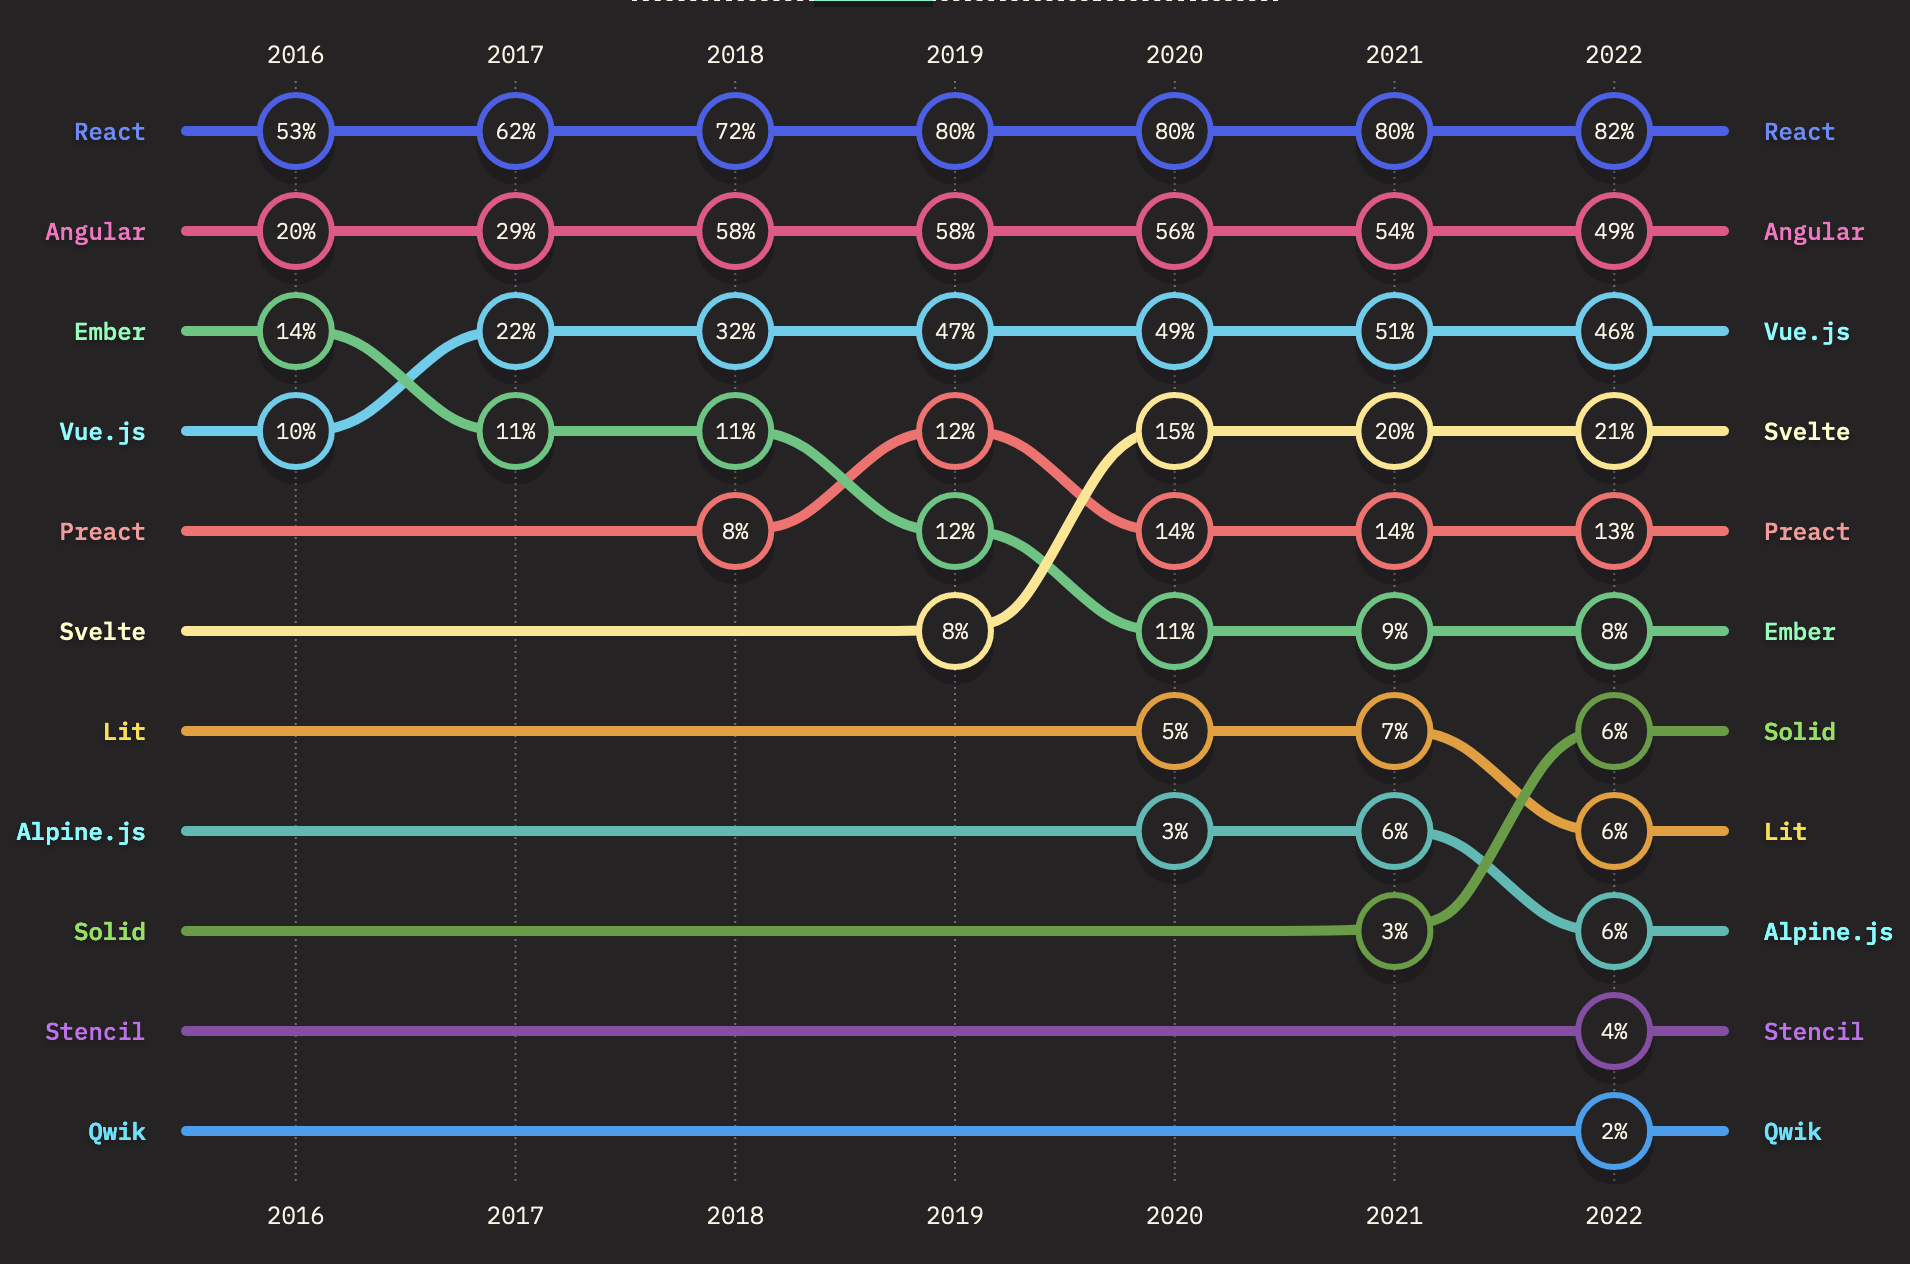
\includegraphics[scale=0.4]{04_Artefakte/01_Abbildungen/stateofjs-usage-frontend-frameworks-2022}
    \caption[Most used frontend frameworks in 2022]{State of JS: Most used frontend frameworks in 2022 \parencite{mostUsedFrontendFrameworks22}\protect}
    \label{fig:mostUsedFrameworks}
\end{figure}

\emph{React}\footnote{\url{https://react.dev}}, developed by Facebook and maintained by its successor Meta, has become the most widely used tool for building \ac{SPA}s.
It is steadily leading the rankings for most used frontend frameworks both in the Stack Overflow~\parencite{stackOverflowPollWebFrameworks23} and the State Of JS~\parencite{mostUsedFrontendFrameworks22} polls.
By definition, it is not a framework but a \ac{UI} library that relies on other extensions to support state management, routing and deployment functionality.
Although it is not a framework itself, there are existing frameworks like Next.js\footnote{\url{https://nextjs.org/}} for the web and ReactNative\footnote{\url{https://reactnative.dev/}} for building mobile apps using native functionality.
React makes use of \ac{JSX}, which allows directly mixing inline \ac{HTML} with the \ac{JS} or \ac{TS} source code.

\emph{Vue}\footnote{\url{https://vuejs.org/}} was developed by Evan You and is maintained by an international team of individuals.
It had a relatively marginal presence in the US and Europe in the first years after its inception.
This can be partially attributed to its origin in China, as most of its supporting modules were localised in Chinese.
Over the years, it grew in popularity and received more international support, eventually overcoming the language barrier.
Unlike React, it is billed as a \textquote{progressive framework} that provides fundamental functionality for building reactive components but also accommodates more complex use-cases~\parencite{vueProgressiveFramework}.
Vue builds on standard \ac{JS} or \ac{TS}, \ac{HTML} and \ac{CSS} to create components, recommending a simple template mechanism mixed with reactive substitutions.
However, it also supports using \ac{JSX} for specifying inline \ac{HTML} within \ac{JS}.
As with React, there are extensions and frameworks like Quasar\footnote{\url{https://quasar.dev}} and Nuxt\footnote{\url{https://nuxt.com}} that enable more sophisticated workflows for application development and deployment.

\emph{Angular}\footnote{\url{https://angular.io/}} was initially released by Google in 2010 as AngularJS and officially discontinued in 2022.
A completely overhauled version 2 was released in 2016 and is maintained by Google.
It differs from React and Vue in that it is a complete framework containing everything required to build and deploy an application, and it explicitly recommends \ac{TS} as a programming language.
The framework is also less flexible because it is more opinionated and has its own set of best practices baked into the framework\textquotesingle s structure.

\section{Backend frameworks}
\label{sec:backend-frameworks}

The \emph{Express}\footnote{\url{https://expressjs.com}} framework provides the basic functionality to create web servers, including routing and middleware functionality.
TJ Holowaychuk developed it in 2010 and sold it to StrongLoop~\parencite{expressJsStrongLoop}, which IBM subsequently acquired~\parencite{expressJsStrongLoopIbm}.
It is currently under the stewardship of the OpenJS Foundation~\parencite{expressJsNodeFoundation}.
Express has become the de facto standard for building web services in JS, leading the ranking in the State of JS survey~\parencite{mostUsedBackendFrameworks22}.
Although it contains the necessary parts to create a web service, it does not enforce a specific architecture, which can be problematic for maintaining a robust application structure.
For developers who prefer a more explicit structure, various other frameworks that add more opinionated structures or extensions are built on top of it.

Billed as a successor to Express, \emph{Koa}\footnote{\url{https://koajs.com}} is developed by the team behind Express.
It aims to provide a more robust and minimalistic iteration of the middleware-based architecture of Express.
Like Express, it allows for building a service from scratch in free form but is also the basis for other, more explicitly structured frameworks.

Other frameworks and a more stringent and structured application structure might be more desirable for complex applications.
Numerous \ac{JS} frameworks, some based on Express or Koa, and others that provide their own basis for routing.
To review all possible options is beyond the scope of this study.
In the following, three frameworks are selected for their specific nature related to popularity and stability, with an explicit focus on real-time applications.

\begin{table}[ht]
\centering
\caption{State of JS survey: Most used backend frameworks \parencite{mostUsedBackendFrameworks22}}
\label{tab:backendFrameworksRanking}
\begin{tabular}[t]{lcc}
\toprule
Framework & \% of question respondents\\
\midrule
Nest & 30.2\\
Feathers & 8.8\\
Meteor & 2.7\\
\bottomrule
\end{tabular}
\end{table}


\emph{Nest}\footnote{\url{https://nestjs.com}} is a backend framework for developers looking for a more strictly opinionated and robust setup than Express, e.g.\ for enterprise applications.
It follows a modular concept, making dependencies available to the services via injection.
Multiple database options exist, and transports can be both \ac{HTTP} and WebSockets.
There are \ac{CLI} scripts that enable automatic generation of boilerplate application code, and the language used to build Nest applications is TypeScript.
It ranks second among the most-used backend frameworks in the State of JS survey~\parencite{mostUsedBackendFrameworks22}.

The \emph{Feathers}\footnote{\url{https://feathersjs.com}} framework takes a different approach, making few assumptions about the specific application structure.
It uses aspect-oriented programming, a service-centric architecture and before-, after- and around-hooks (so-called \textquote{cross-cutting concerns}) for the services that modify basic behaviour or add functionality.
There are adapters for a wide range of databases and authentication methods.
The framework has a dedicated concept of channels that enable real-time functionality and messaging to clients.
Real-time transports are abstracted and can be deployed using Socket.IO or standards-compliant µWebSockets (see \autoref{sec:webstandards}). It also provides a \ac{CLI} to generate application code in \ac{JS} or \ac{TS}.
Feathers started as a hobby project by David Luecke and Eric Kryski in 2013~\parencite{feathersFrameworkHistory} and is currently maintained by David Luecke and a community of individual contributors.
It still ranks in the lower percentages in the State of JS survey~\parencite{mostUsedBackendFrameworks22} but almost doubled that percentage from the previous one in 2021~\parencite{mostUsedBackendFrameworks21}.

\emph{Meteor}\footnote{\url{https://www.meteor.com}} focuses explicitly on real-time applications using WebSockets.
The framework is an outlier because while its core is open-source, other parts are proprietary code.
Nonetheless, it should be mentioned because it has been around for over ten years and uses WebSockets exclusively.
It was released in 2012 by a startup company, immediately received venture capital funding from Andreessen Horowitz and was eventually sold to Tiny Capital in 2019~\parencite{meteorSaleTinyCapital}.
The framework primarily uses MongoDB as a database system and initially provided its own package manager and ecosystem, build system, and template system based on Mustache.
Meanwhile, this exclusive strategy has been abandoned in favour of adopting the Node Package Manager.
Still, it seems to be subject to debate regarding its ease of use versus its \textquote{growing pains} and related trouble with wide adoption~\parencite{meteorDiscussionYCombinator}.

\section{Databases}
\label{sec:databases}

\begin{table}[ht]
\centering
\caption{Stack Overflow Developer Survey 23: The top three multi-user databases \parencite{stackOverflowPollDatabases23}}
\label{tab:stackOverflowDatabasesRanking}
\begin{tabular}[t]{|l|r|r|}
\toprule
Database & \% of all question respondents & Stars on GitHub (k)\\
\midrule
\cite{githubPostgreSql} & 45.55 & 14\\
\cite{githubMySql} & 41.09 & 9.9\\
\cite{githubMongoDb} & 25.52 & 25\\
\bottomrule
\end{tabular}
\end{table}

\emph{PostgreSQL}\footnote{\url{https://www.postgresql.org}} is a very widely used database which uses a table-based data topology and implements \ac{SQL} for interaction with the database and its contents.
The relatively rigid database schema provides a solid structure for data storage and retrieval but, on the other hand, requires migrations to be written to transition from one database structure version to another.
It has an extensive feature set supporting complex data structures, \ac{GIS} data and data structured in \ac{JSON} format.
Developed in the 1980s at the University of California and switched to the \ac{SQL} in the 90s, it has remained a popular choice for enterprise and small-scale use.

Similar to PostgreSQL in that it also uses \ac{SQL}, \emph{MySQL}\footnote{\url{https://www.mysql.com}} supports many of the features of PostgreSQL, but has an overall smaller feature set.
It was initially developed in the 1990s by the private Swedish company MySQL AB and was forked as a completely open-source version in 2009 and renamed MariaDB\footnote{\url{https://mariadb.org}}.
It is still a popular choice, especially for smaller web projects that don\textquotesingle t need the extra functionality and value its relatively simple setup.

\emph{MongoDB}\footnote{\url{https://www.mongodb.com}} is a document store database that is designed to hold large amounts of unstructured data.
It has its own query language and features aggregation functionality that allows map/reduce and transformation operations or resolving of relations on the data before being sent to the client.
Although it uses the \ac{NoSQL} paradigm and allows storing documents of any kind in a collection, it eventually added the option of using schemas for validation.
It was initially released as open-source in 2009, then was put under a proprietary license in 2018, but remains available to be used for free with limited support.

\section{Application deployment}
\label{sec:application-deployment}

\emph{Containerisation}, in the context of computing infrastructure, refers to the~\textquote[\cite{containerisationDefinition}]{packaging of software code with just the operating system (OS) libraries and dependencies required to run the code to create a single lightweight executable—called a container—that runs consistently on any infrastructure.} It was popularised through the release of the Docker Engine\footnote{\url{https://www.docker.com}}, an open-source project devoted to creating an industry standard for application containerisation~\parencite{dockerRelease}.
The Docker team eventually launched the \ac{OCI} in 2015, which serves as \textquote{a lightweight, open governance structure (project), formed under the auspices of the Linux Foundation, for the express purpose of creating open industry standards around container formats and runtimes.} It subsequently received Docker's container runtime and format as a donation, which was released as runC version 1.0 in 2020~\parencite{openContainerInitiative}.
It has recently become the de facto standard for packaging and delivering applications in web development and beyond.
GitHub reports that~\textquote[\cite{stateOfTheOctoverse23}]{in 2023, 4.3 million public and private repositories used Dockerfiles --- and more than 1 million public repositories used Dockerfiles for creating containers.}

\emph{Container orchestration} builds on the concept of containerisation. \textquote[\cite{orchestrationDefinition}]{Container orchestration automates the provisioning, deployment, networking, scaling, availability, and lifecycle management of containers.} The concept first gained popularity as Docker \textquote{swarm mode}, a functionality of the Docker software. Still, its most successful instance so far is the software package Kubernetes\footnote{\url{https://kubernetes.io}}, which originated at Google in late 2013~\parencite{kubernetesHistory} and went on to be included in the \ac{CNCF}, a project by the Linux Foundation, that~\textquote[\cite{cloudNativeComputingFoundation}]{aims to advance the state-of-the-art for building cloud-native applications and services}.
It can be extended, highly customised and deployed on anything from an embedded device to a large-scale cloud infrastructure, providing a versatile deployment and management tool for many application infrastructures.
